En la carpeta \texttt{mediciones} se encuentran los archivos de salida correspondientes a cada
experimento. Por cada uno, se adjunta un archivo \texttt{README.txt} con la información conocida
sobre la red en cuestión y otro arhivo \texttt{exceptions.txt} que describe los paquetes sin tipo
capturados. Los nombres de los experimentos denotan el tipo de red, el tipo de conexión y la
duración del experimento en minutos.

% \subsection{Experimento 1: Red hogareña, cableada, 10 mintos}
\subsection{Experimento 1: Red hogareña}
\subsubsection{Medición cableada}

\begin{center}
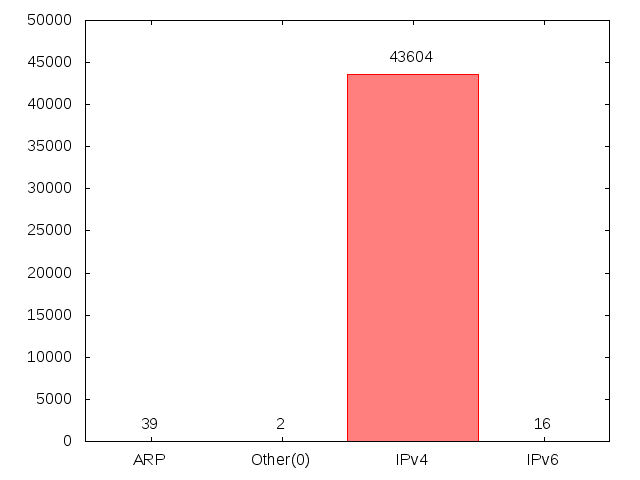
\includegraphics[width=8cm]{../mediciones/home-eth-10/home-eth-10Protocolos.png}
\end{center}

En este gráfico podemos observar que ARP se usa muy poco en relación con IP. Imaginamos que es porque hay pocos nodos en la red y se aprende rápido la configuración de la red.
En cuanto a la diferencia entre los distintas versiones de IP, nuestra hipótesis es que en general vamos a encontrar más paquetes IPv4 que IPv6 ya que todavía no se migró a la versión 6 del protocolo IP.
Dicha hipótesis se ve confirmada en este gráfico ya que la relación entre ambas versiones del protocolo es aproximadamente 2725 a 1 a favor de la versión 4.
Es claro que el tipo $0x0800$ correspondiente al protocolo IPv4, es un símbolo distinguido de la fuente \textbf{S} ya que es el que más aparece,
es decir que es el que tiene mayor probabilidad. El resto de los símbolos tienen frecuencias similares y mucho menores a la de $0x0800$.

\begin{figure}[!h]
\centering
\begin{minipage}{8cm}
  \centering
  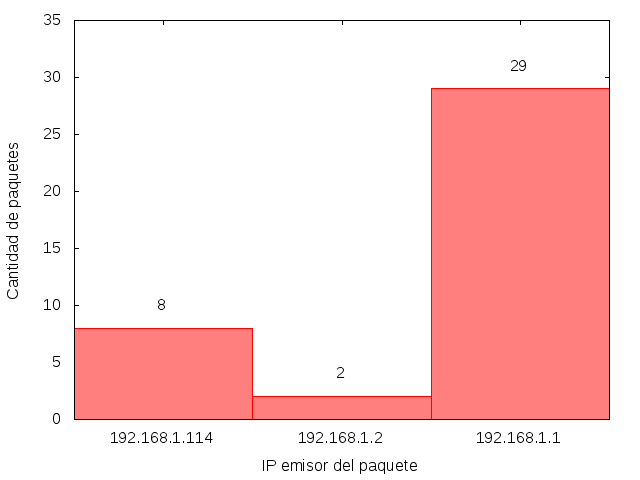
\includegraphics[width=8cm]{../mediciones/home-eth-10/home-eth-10IpsSrcArp.png}
\end{minipage}%
\begin{minipage}{8cm}
  \centering
  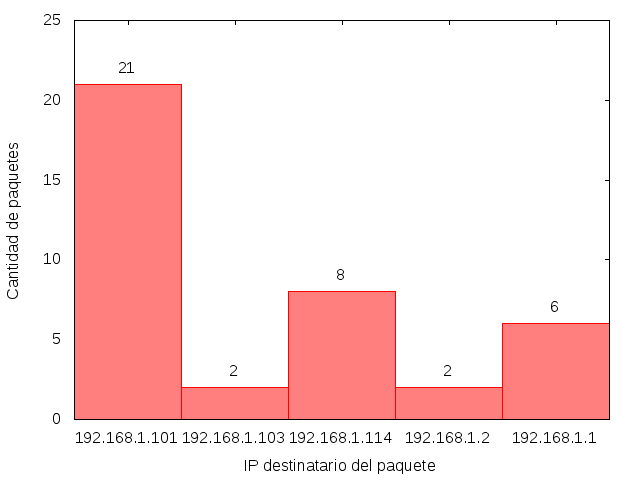
\includegraphics[width=8cm]{../mediciones/home-eth-10/home-eth-10IpsDstArp.png}
\end{minipage}
\end{figure}

Vemos que para este experimento no tiene sentido considerar la IP del emisor de un paquete para identificar a los nodos de la red ya que sólo tres direcciones
(la de la computadora que está ejecutando el experimento y las de los dos routers) son visibles. Esto tiene sentido al considerar que la computadora que
está ejecutando el experimento está conectada al router principal (con dirección \textbf{192.168.1.1}) a través de un cable ethernet, por lo que los paquetes emitidos
por otros hosts no deberían llegar hasta este equipo. En cuanto a los destinatarios de los paquetes, vemos que el router no representa un símbolo distinguido
como sí lo hacía en la fuente de basada en emisores.

\begin{center}
\begin{tabular}{|c||c|}
\hline
Entropía de los protocolos & 0.0157726691884  \\
\hline
Entropía de las IPs origen de ARP & 1.00639070966  \\
\hline
Entropía de las IPs destino de ARP & 1.80467296546 \\
\hline
\end{tabular}
\end{center}

\subsubsection{Medición inalámbrica}

\begin{center}
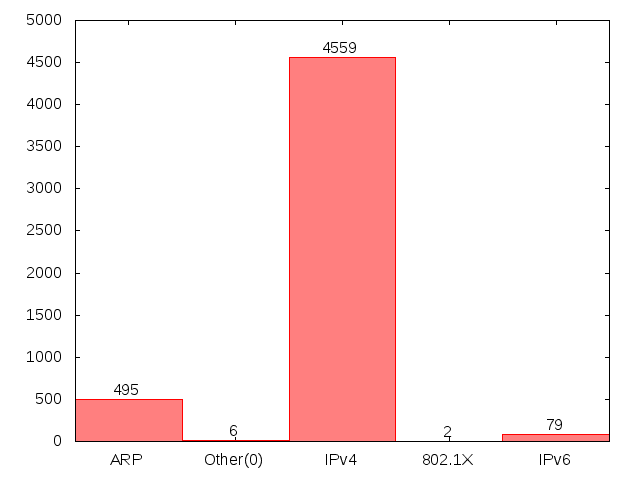
\includegraphics[width=8cm]{../mediciones/home-wfi-10/home-wfi-10Protocolos.png}
\end{center}

Otra vez se ve la superioridad de la versión 4 del protocolo IP, no sólo sobre la versión 6 del mismo protocolo, sino sobre el resto de los protocolos.
Sin embargo, la proporción es mucho menor. Al comparar este gráfico con el del experimento anterior, notamos dos cambios significativos. Por un lado la cantidad
de paquetes de tipo IPv4 es casi 10 veces menor. Por otro lado la cantidad de paquetes de tipo ARP y de tipo IPv6 se multiplicaron varias veces. Si consideramos
que la duración fue de 10 minutos para ambos experimentos, llama la atención esta diferencia. Como se puede ver en la siguiente tabla, los paquetes Ipv4 pasaron
de ocupar el 99.9\% de los paquetes capturados a ocupar el 88.7\%. Los de tipo IPv6 pasaron del 0.04\% al 1.54\% y los de tipo ARP pasaron del 0.09\% al 9.63\%.

\begin{center}
\begin{tabular}{|c||c|c|}
\hline
Protocolo & Red cableada & Red Wifi \\
\hline
ARP & 0.09\% & 9.63\% \\
\hline
IPv4 & 99.87\% & 88.68\% \\
\hline
IPv6 & 0.04\% & 1.54\% \\
\hline
Otros & 0.01\% & 0.16\% \\
\hline
\end{tabular}
\end{center}

\begin{figure}[!h]
\centering
\begin{minipage}{8cm}
  \centering
  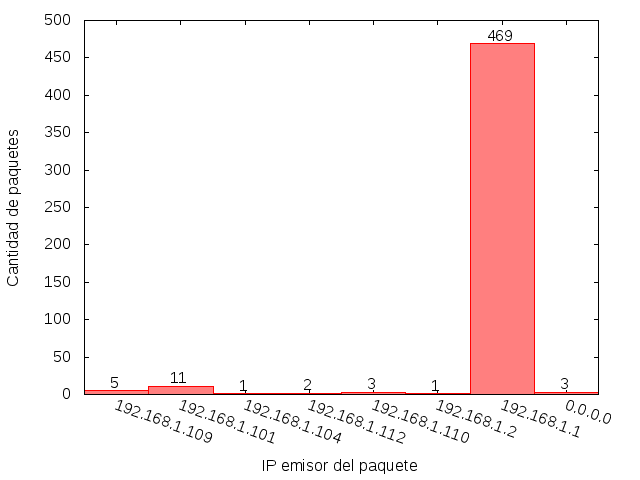
\includegraphics[width=8cm]{../mediciones/home-wfi-10/home-wfi-10IpsSrcArp.png}
\end{minipage}%
\begin{minipage}{8cm}
  \centering
  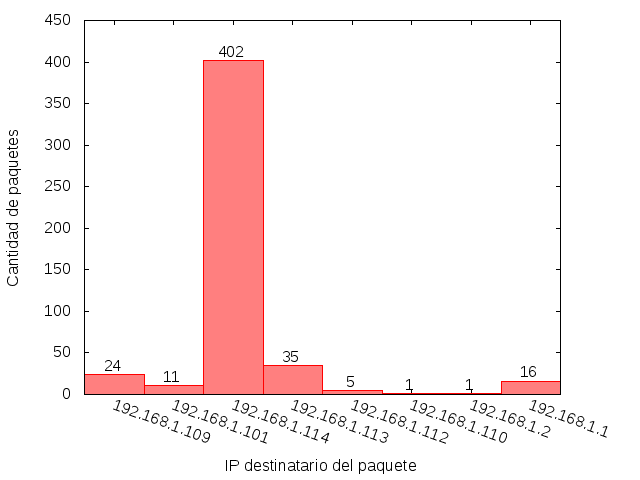
\includegraphics[width=8cm]{../mediciones/home-wfi-10/home-wfi-10IpsDstArp.png}
\end{minipage}
\end{figure}

En cada uno de estos gráficos encontramos un nodo distinguido. Del lado de los emisores, la dirección IP distinguida corresponde al
router principal de la red, mientras que el nodo al que más paquetes van dirigidos es el host que ejecuta el experimento. El resto
de las direcciones mantiene una baja frecuencia de envío y recepción de paquetes. Otro punto a notar es la aparición de la dirección
\textbf{0.0.0.0} como emisor de 3 paquetes.

\begin{center}
\begin{tabular}{|c||c|}
\hline
Entropía de los protocolos & 0.5871665762  \\
\hline
Entropía de las IPs origen de ARP & 0.420338347182  \\
\hline
Entropía de las IPs destino de ARP & 1.11098133367 \\
\hline
\end{tabular}
\end{center}


\subsection{Experimento 2: Red pública}
\subsubsection{Medición 10 minutos}

\begin{center}
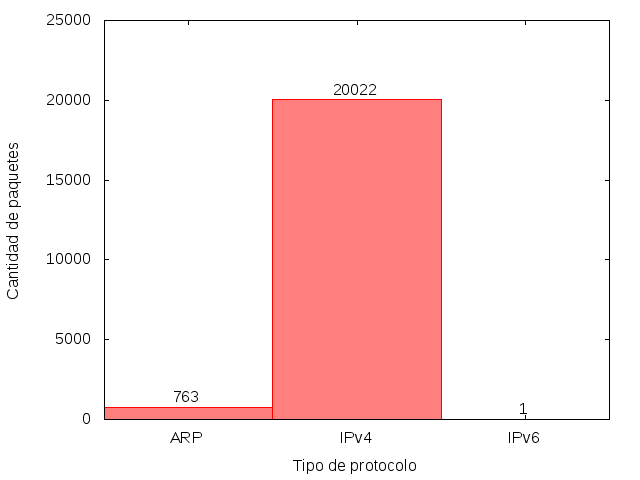
\includegraphics[width=8cm]{../mediciones/altop-wifi-10/altop10Protocolos.png}
\end{center}

Seguimos viendo en esta red que el protocolo IPv4 es el más utilizado para el envío de paquetes. Es particularmente notoria la escasa
cantidad de paquetes de tipo IPv6, mucho menor que en la red hogareña del experimento anterior. Sí se incrementa la cantidad de paquetes
de tipo ARP en la misma cantidad de tiempo, respecto a la red hogareña. Esto puede deberse a que la red pública es considerablemente mayor.

\begin{center}
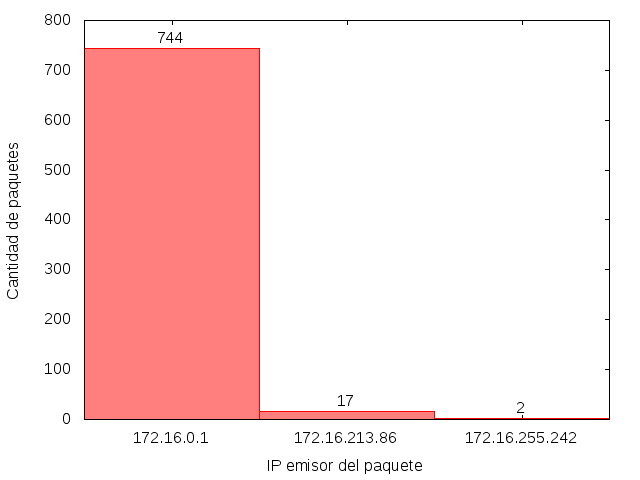
\includegraphics[width=8cm]{../mediciones/altop-wifi-10/altop10IpsSrcArp.png}
\end{center}

En este caso nos encontramos con un comportamiento inesperado. Más del 97\% de los paquetes capturados fueron emitidos por una misma dirección
IP, que podemos suponer que es el router. Por otro lado, sólo pudieron identificarse 3 direcciones IP distintas en la red, a diferencia de lo
que había sucedido en la red hogareña, en la que se pudieron identificar varios nodos más. Claramente, la IP \textbf{172.16.0.1} es un símbolo
distinguido de la fuente.

\begin{center}
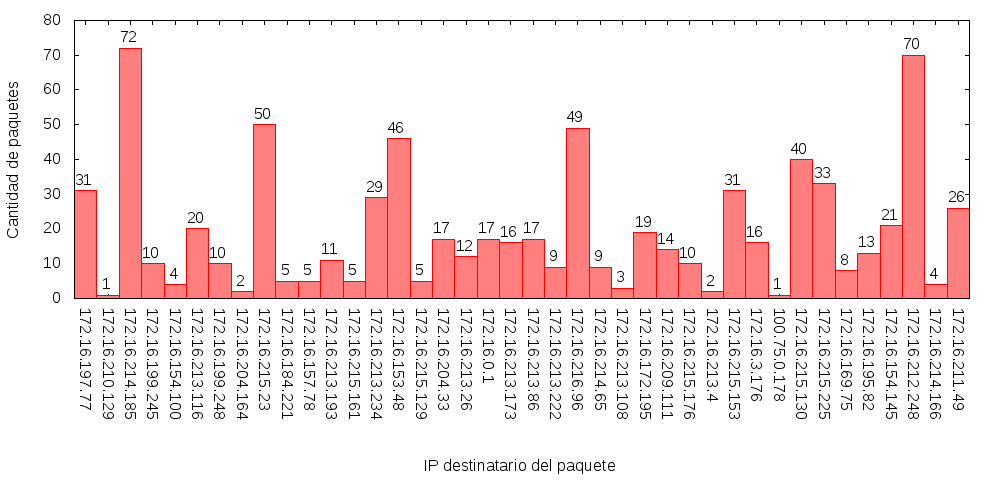
\includegraphics[width=16cm]{../mediciones/altop-wifi-10/altop10IpsDstArp.png}
\end{center}

Este gráfico muestra algo más parecido a lo esperado en cuanto a la cantidad de nodos identificados. Lo que es incierto es la razón por la cual
los paquetes son dirigidos a tantos nodos distintos pero emitidos por un grupo reducido.

\begin{center}
\begin{tabular}{|c||c|}
\hline
Entropía de los protocolos & 0.227743354201  \\
\hline
Entropía de las IPs origen de ARP & 0.180229910313  \\
\hline
Entropía de las IPs destino de ARP & 4.77276412705 \\
\hline
\end{tabular}
\end{center}


\subsubsection{Medición 60 minutos}

\begin{center}
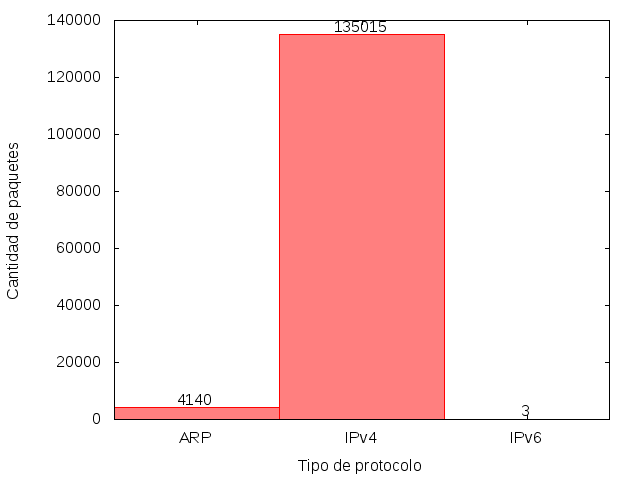
\includegraphics[width=8cm]{../mediciones/altop-wifi-60/altop60Protocolos.png}
\end{center}

\begin{center}
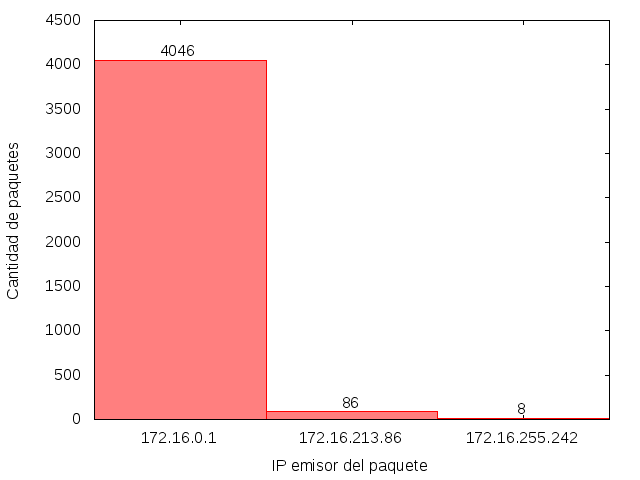
\includegraphics[width=8cm]{../mediciones/altop-wifi-60/altop60IpsSrcArp.png}
\end{center}

\begin{center}
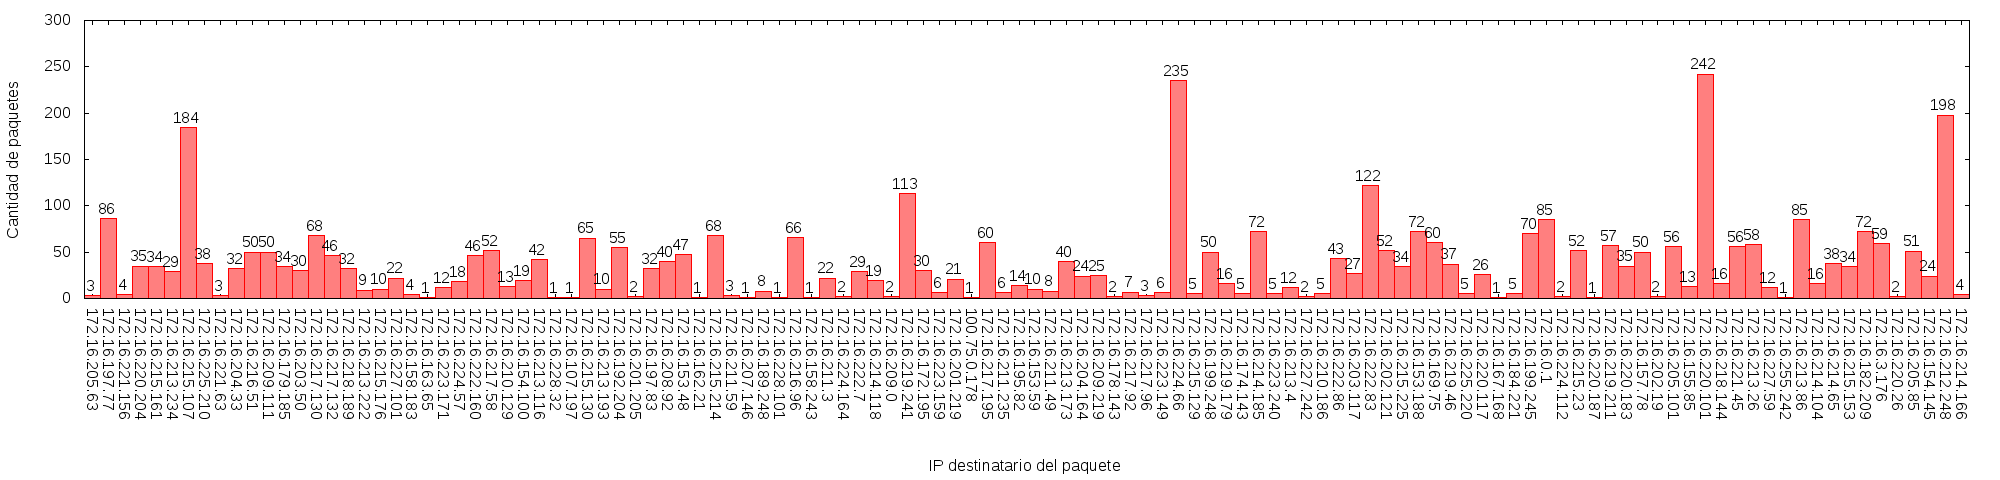
\includegraphics[width=16cm]{../mediciones/altop-wifi-60/altop60IpsDstArp.png}
\end{center}

Para poder observar este gráfico mejor, lo agregamos en el Apéndice, en la sección \ref{exp2_60_big}.


\begin{center}
\begin{tabular}{|c||c|}
\hline
Entropía de los protocolos & 0.193502700102 \\
\hline
Entropía de las IPs origen de ARP & 0.1659063338  \\
\hline
Entropía de las IPs destino de ARP & 6.07060528117 \\
\hline
\end{tabular}
\end{center}


\subsection{Experimento 3: Red laboral}
\subsubsection{Primera medición 60 minutos}

\begin{figure}[!h]
\centering
\begin{minipage}{8cm}
  \centering
  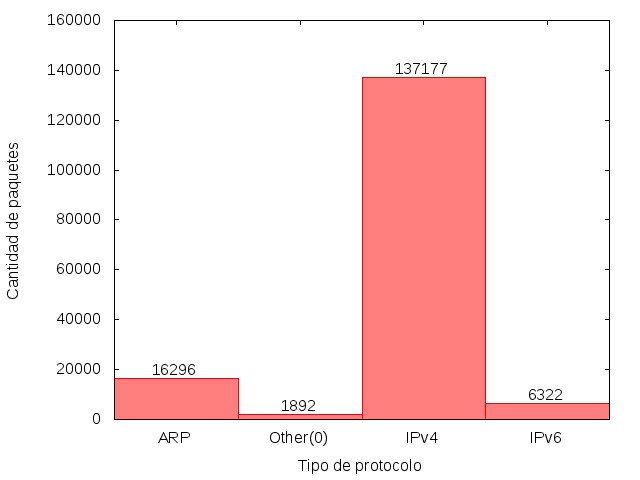
\includegraphics[width=8cm]{../mediciones/job1/type.png}
\end{minipage}%
\begin{minipage}{8cm}
  \centering
  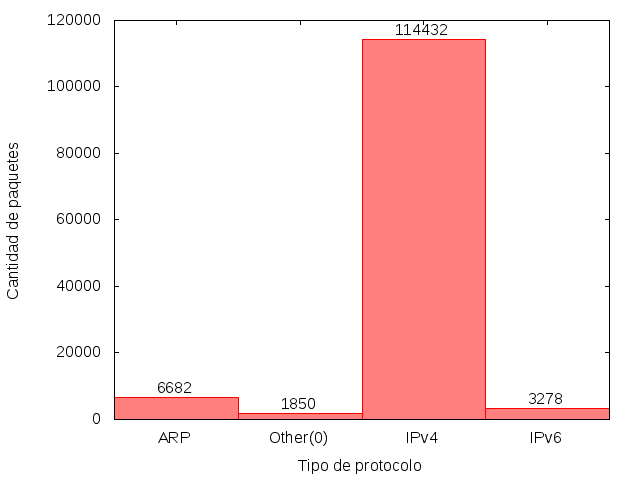
\includegraphics[width=8cm]{../mediciones/job2/type.png}
\end{minipage}
\end{figure}

\begin{center}
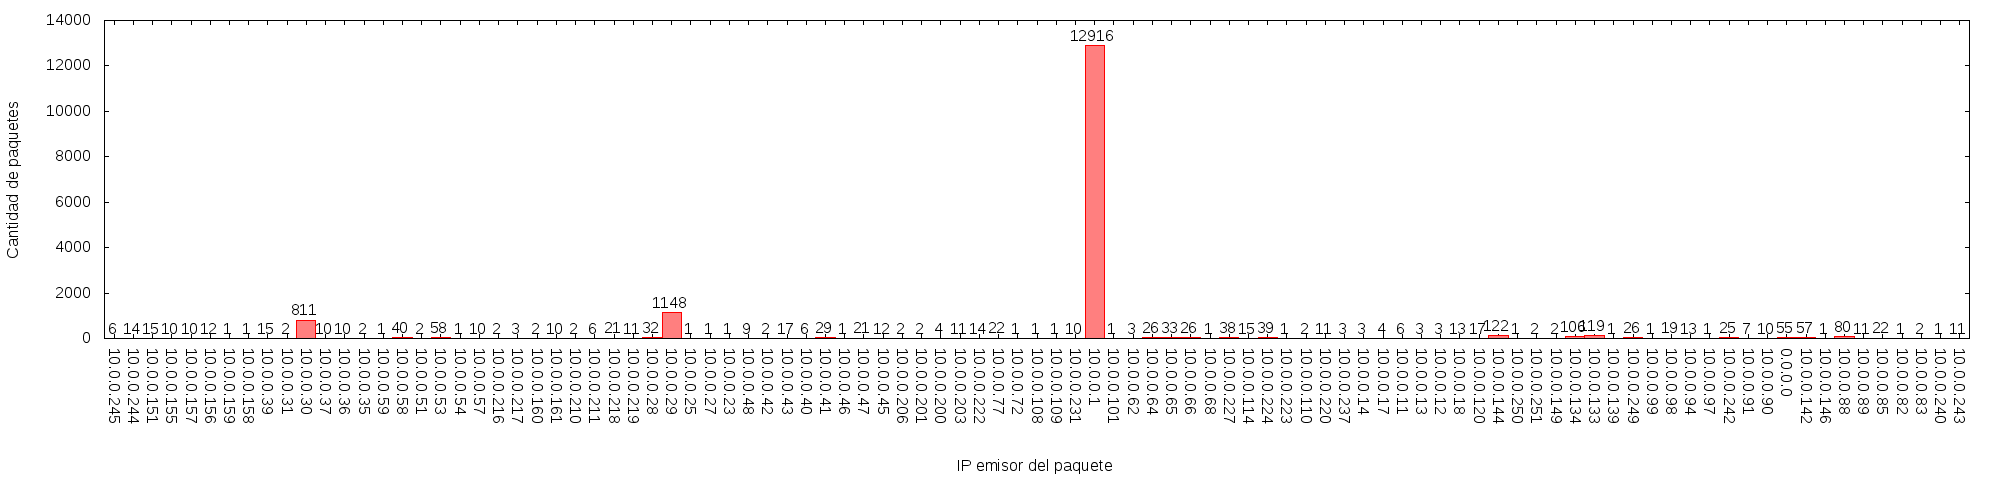
\includegraphics[width=16cm]{../mediciones/job1/src.png}
\end{center}

\begin{center}
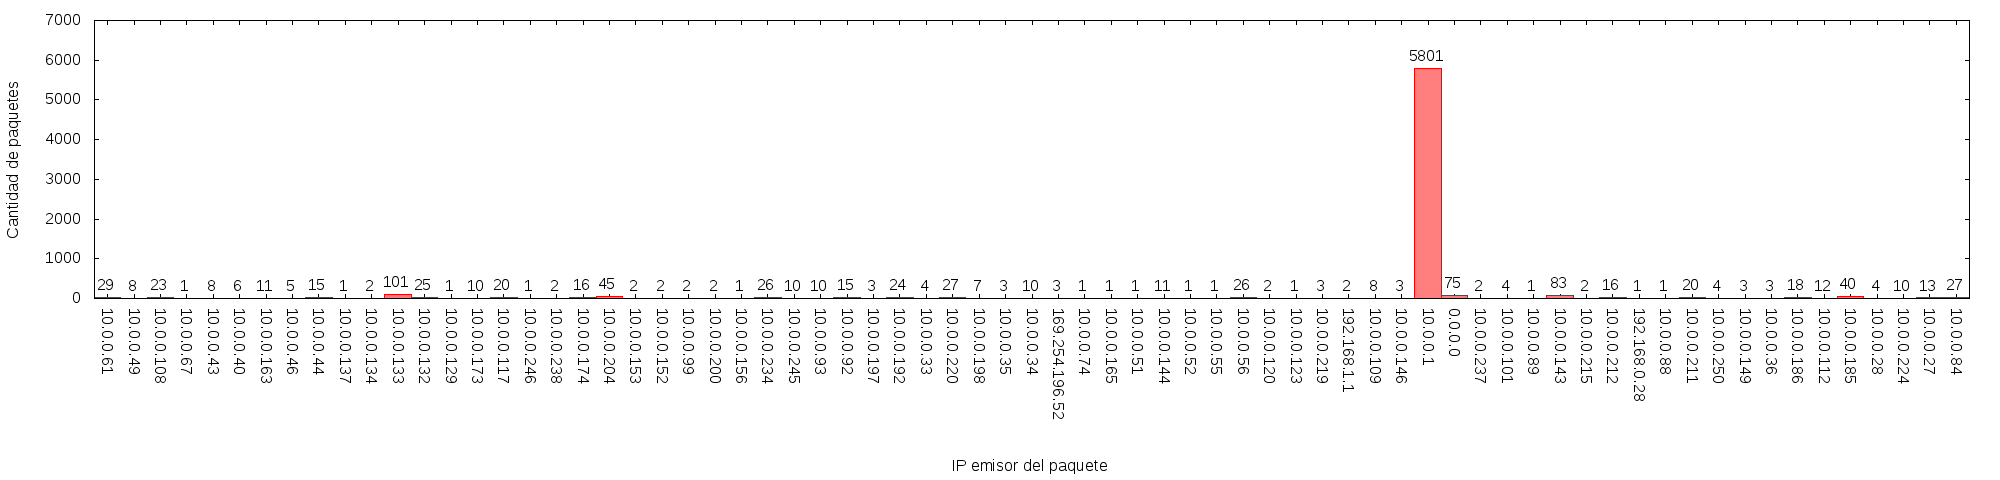
\includegraphics[width=16cm]{../mediciones/job2/src.png}
\end{center}

\begin{center}
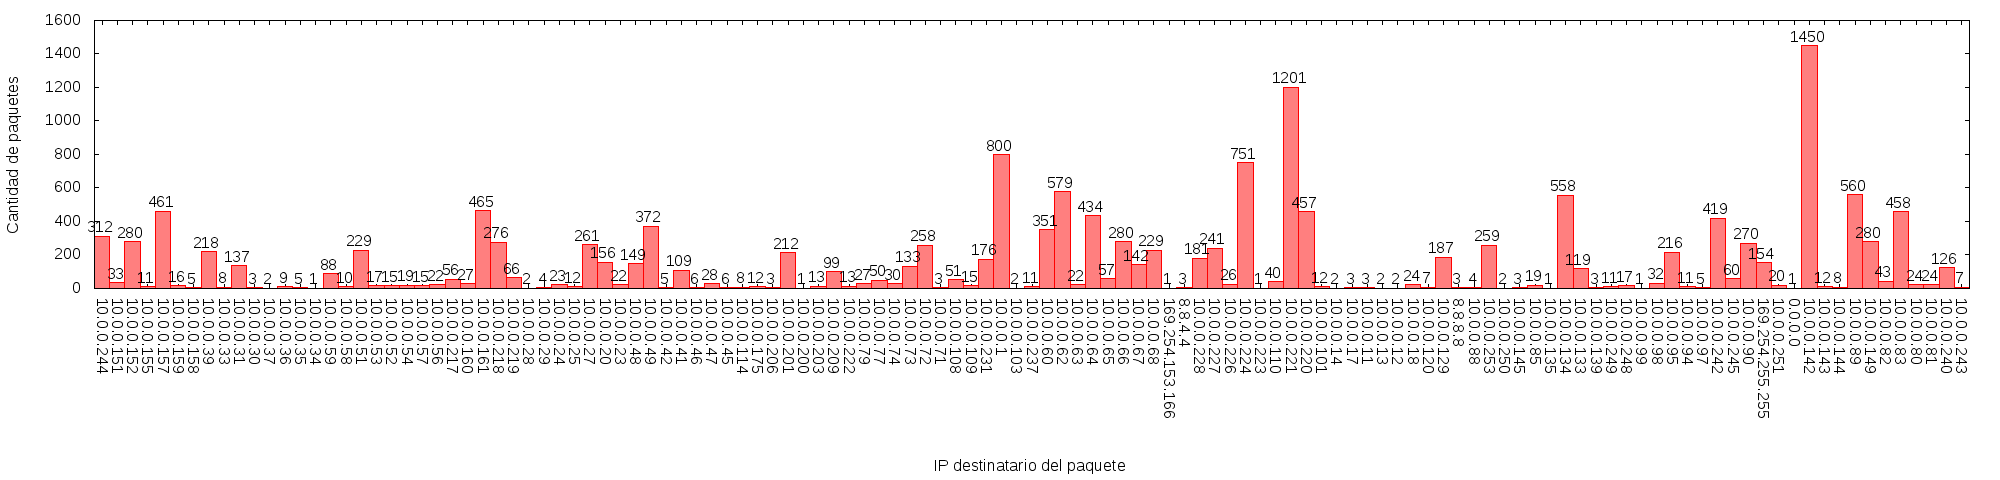
\includegraphics[width=16cm]{../mediciones/job1/dst.png}
\end{center}

\begin{center}
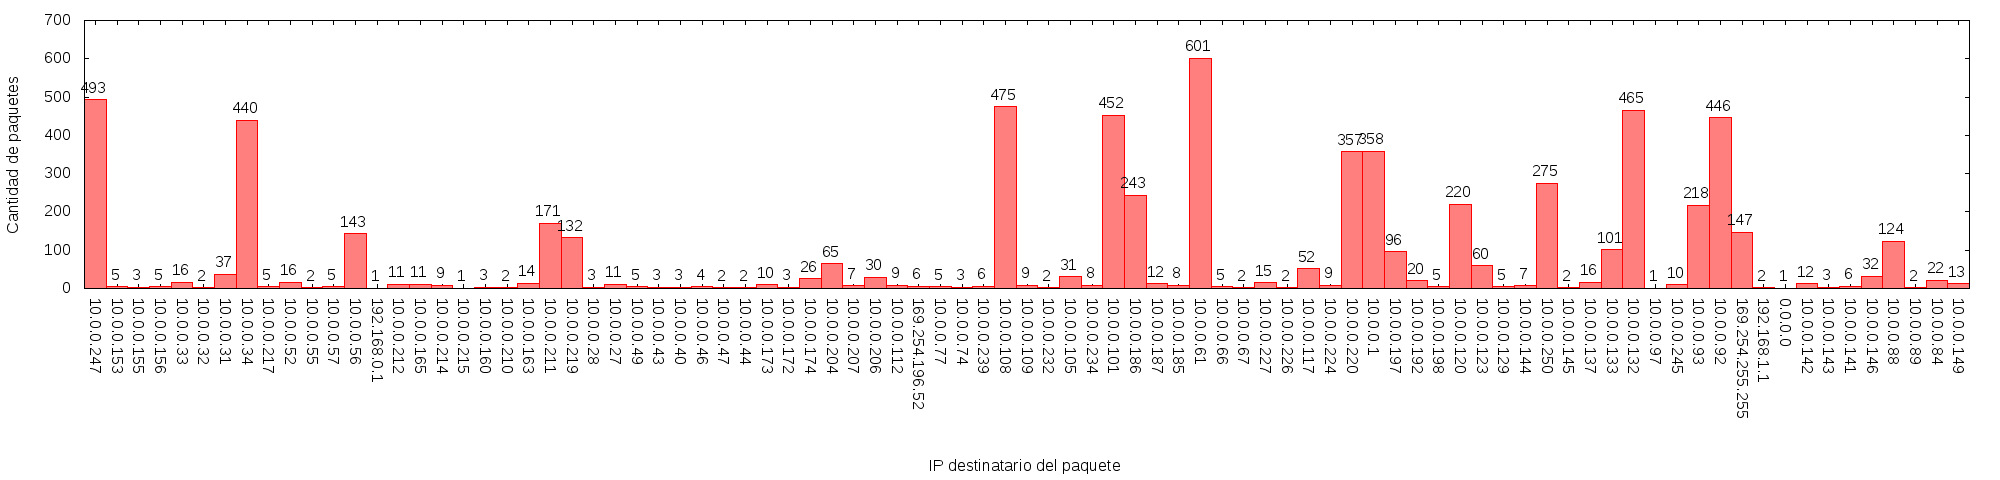
\includegraphics[width=16cm]{../mediciones/job2/dst.png}
\end{center}

\begin{center}
\begin{tabular}{|c||c|c|}
\hline
Entropía & Medición 1 & Medición 2 \\
\hline
Entropía de los protocolos & 0.792831613911 & 0.578907674515 \\
\hline
Entropía de las IPs origen de ARP & 1.53247970384 & 1.23402710535 \\
\hline
Entropía de las IPs destino de ARP & 5.53038672313 & 4.7457277713 \\
\hline
\end{tabular}
\end{center}





\subsection{Entropía}

\begin{center}
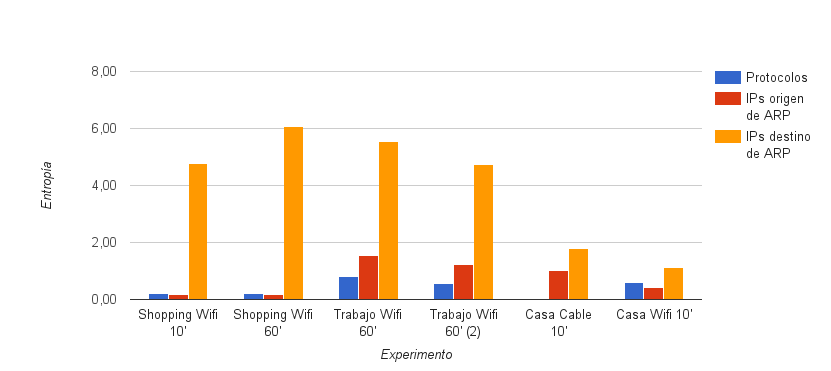
\includegraphics[width=14cm]{../mediciones/entropias.png}
\end{center}
